\chapter{Experiments}\label{sec:experiments}
The first important thing that needs to be discussed before describing experiments is machine on which experiments have been performed. Experimental machines properties looks as follows:
\begin{itemize}
    \item Operating system: Windows 10 Professional,
    \item Processor: Intel(R) Core i5-11400F
    \begin{itemize}
        \item 11th generation,
        \item 2.60GHz
    \end{itemize}
    \item RAM: 16 GB DDR4,
    \item Graphical card: NVIDIA GeForce GTX 970,
    \item Hard drive: 500 GB SSD.
\end{itemize}
Those parameter can be changed but it is important to remember that used game tree structure is very memory consuming and neural network training require a lot of computation power. It is recommended to use specified parameters of higher. Last important thing to mention is the fact that result application has been created for Windows operating system only and wasn't tested on other operating systems.

\section{Methodology}\label{sec:methodology}
Performed tests was divided into three sets of tests:
\begin{description}
    \item[Neural network training] this set of tets was based on training created neural network instances. It allows for finding the most optimal values of learning rate parameter. After that, AI instances were tested for number of iterations (epochs) require to get the best accuracy and number of data require for training. More information about datasets used for training can be found in section \ref{sec:data-sets}.
    \item[Manual testing] this set of tests relied on playing against AI instances in ,,player vs AI'' scenario. This set of tests covered test case in which player play against trained and untrained AI instance. Important thing to mention is the fact that this set of tests required both neural networks to be trained on the same size of data set. Otherwise, experiment would be unreliable.
    \item[Automated testing] this set of test was performed in ,,AI vs AI'' scenario. The main goal of this testing was to perform small ,,tournament'' to check which AI instance performs better. Similarly to te manual testing, this set of test has been performed with trained and untrained neural networks. Both neural networks was trained with the same data set.
\end{description}

\subsection{Chess application}
To perform mentioned tests, it was necessary to have application that allows for chess game. Application has been created and while starting it it is possible to specify which execution scenario needs to be performed. Because application uses command line interface, execution configuration is passed by input parameters. By specifying \texttt{--exScenario} parameter, application can be started in one of 3 modes:
\begin{itemize}
    \item parameter value: \texttt{0} - application will start in mode ,,player vs player'',
    \item parameter value: \texttt{1} - application will start in mode ,,player vs AI'',
    \item parameter value: \texttt{2} - application will start in mode ,,AI vs AI''.
\end{itemize}
Default value of this parameter is set on \texttt{0}. If \texttt{--exScenario} parameter will have value \texttt{1} or \texttt{2} application will ask for game tree limit to be specified (\hyperref[fig:setting-game-tree-depth]{fig. \ref*{fig:setting-game-tree-depth}}). If user won't specify this parameter, its value will be set on $3$.
\begin{figure}
    \centering
    \begin{mdframed}
    \VerbatimInput{dependencies/documents/Setting_Game_Tree_Depth.txt}
    \end{mdframed}
    \caption{Menu allowing game tree depth specification.}
    \label{fig:setting-game-tree-depth}
\end{figure}

\subsubsection{Chess application - manual control}
Choosing proper execution mode for the application, have impact on method of controlling application. If \texttt{--exScenario} parameter will have value \texttt{0} or \texttt{1}, application will show proper menu presented on \hyperref[fig:application-main-page]{fig. \ref*{fig:application-main-page}}
\begin{figure}
    \centering
    \begin{mdframed}
    \VerbatimInput{dependencies/documents/Application_Main_Page.txt}
    \end{mdframed}
    \caption{Application main page.}
    \label{fig:application-main-page}
\end{figure}
Application main menu allows user to choose one of three options:
\begin{description}
    \item[New game] (command \texttt{N} / \texttt{n}) which reset all environment configurations and start new, fresh game. Choosing this option allows to set new game tree depth.
    \item[Move] (command \texttt{M} / \texttt{m}) which allows user to perform move. Choosing this option allows to select option \texttt{?} which print out information about legal moves syntax.
    \item[Quit] (command \texttt{Q} / \texttt{q}) which close application.
\end{description}
Last thing worth mentioning is move command syntax. For move command to be accepted by the system, it is required to specify horizontal coordinate (a \dots h) first and vertical coordinate (1 \dots 8) second.
\begin{itemize}
    \item \textbf{Syntax: <piece-id><starting-position><ending-position>}
    \item \begin{itemize}[label={}]
        \item where:
        \begin{itemize}[label={}] 
            \item piece-id := \{K -- king, Q -- queen, B -- bishop, N -- knight, R -- rook, P -- pawn\}
            \item starting-position / ending-position := \{a1\dots h8\}
        \end{itemize} 
        \item description: Performs traditional move. Traditional capturing is also handled by this command.
        \item example: Nb8a6.   
    \end{itemize}
    \item \textbf{Syntax: 0-0}
        \begin{itemize}[label={}]
            \item description: Performs short castling. 
        \end{itemize}
    \item \textbf{Syntax: 0-0-0}
        \begin{itemize}[label={}]
            \item description: Performs long castling. 
        \end{itemize}
    \item \textbf{Syntax: \texttt{P<starting-position>-><piece-id>}}
        \begin{itemize}[label={}]
            \item where:
            \begin{itemize}[label={}]
                \item starting-position := \{a1\dots h8\}
                \item piece-id := \{K -- king, Q -- queen, B -- bishop, N -- knight, R -- rook, P -- pawn\} 
            \end{itemize}
            \item description: Promote pawn to chosen piece.
            \item example: Pb7->Q. 
        \end{itemize}
    \item \textbf{Syntax: \texttt{P<starting-position>x<first-coordinate-ending-position>}}
        \begin{itemize}[label={}]
            \item where:
            \begin{itemize}[label={}]
                \item starting-position := \{a1\dots h8\}
                \item first-coordinate-ending-position := \{a\dots h\} 
            \end{itemize}
            \item describing: Performs en-passant manoeuver.
            \item example: Pc4xd.
        \end{itemize}
\end{itemize}

\subsection{Chess application - automated control}
If \texttt{--exScenario} parameter has value \texttt{2}, application will also show chessboard and capture lists but control will be limited. After each turn, user will be able to continue game or stop it and exit application. This option was implemented to provide infinite games in which both AI instances play on the same level.

\section{Data sets}\label{sec:data-sets}
To train created neural network instances, PGN files were used. Those are text file that contains records of chess games. PGN files consists of basic information about game, sequence of moves performed in this game and final outcome of the game. Example of the PGN file can be found on \hyperref[fig:pgn-example]{fig. \ref*{fig:pgn-example}}.
\begin{figure}
    \centering
\begin{mdframed}
    \VerbatimInput{dependencies/documents/PGN_Example.txt}
\end{mdframed}
    \caption{PGN file example.}
    \label{fig:pgn-example}
\end{figure}
Presented example consists of field ,,Result''. This field contains information about result of the game. To present information about winner, one of the following values can be used:
\begin{itemize}
    \item \texttt{1/2-1/2} - draw,
    \item \texttt{0-1} - black site player win,
    \item \texttt{1-0} - white ste player win.
\end{itemize}


Unfortunately, PGN files in their plain format couldn't been used for training neural networks instances. As it was mentioned in section \ref{sec:ann-architecture}, as an input for neural networks, chessboard representation is used. To make training process possible, gathered PGN files needed to be processed and converted into chessboard situations. For converting PGN files, specially implemented class has been used. This class takes as an input PGN file and convert sequence of moves on respective chessboard situations. After converting sequence of moves, every chessboard situation needed to have evaluation value assigned to it. Evaluation value of each chessboard situation has been calculated using formula:
\begin{equation}\label{eq:evaluation-equation-pgn}
    Ev = sign\left(1/t_c\right),
\end{equation}
where:
\begin{itemize}[label=]
    \item $Ev$ -- evaluation value, $sign$ -- sign of the winning site (if black site ,,-'', if white site ,,+''), $t_c$ -- number of turns to end of the game.
\end{itemize}
In conclusion, every training example consists of chessboard situation and evaluation value. Last thing worth mentioning is the fact that prepared dataset has been divided into train and test set in proportions 70\% and 30\%, respectively.

\section{Results}
Like it can be seen in section \ref{sec:methodology}, tests has been divided into three main parts. To facilitate reading, results description will also be divided into three sections.

\subsection{Neural networks training}\label{sec:neural-network-training}
First test that has been performed in this test set was time consumption in relation to number of processed examples. Because number of epochs is irrelevant to this experiment, all tests runs has been executed with number of epochs equal to $1$. In total, 5 test runs has been performed with data set split ratio of $0.7$ and following data set sizes: $500$, $1000$, $2000$, $5000$ and $10000$. Results of the experiment are shown on \hyperref[fig:training-time-consumpption]{fig. \ref*{fig:training-time-consumpption}}.
% ANN training times: 350examples - 44.4s, 700examples - 85.2s, 1400examples - 171.6s, 3500examples - 429.2, 7000examples - 869.2
% CNN training times: 350examples - 62.5s, 700examples - 124.5s, 1400examples - 202.4s, 3500examples - 499.5, 7000examples - 1048.9
\begin{figure}
\centering
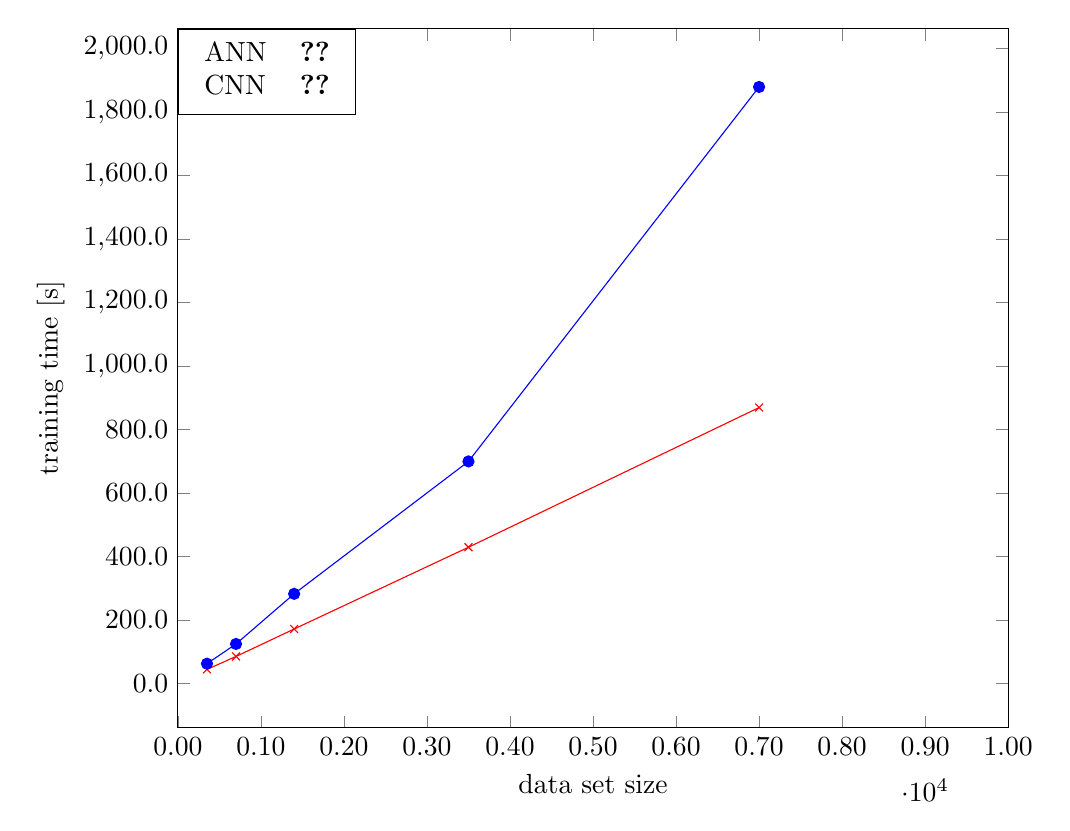
\begin{tikzpicture}
\begin{axis}[
    name=training-time-consumption,
    xmin=0, xmax=10000,
    % xtick={350, 700, 1400, 3500, 7000},
    width=\textwidth,
    y tick label style={
        /pgf/number format/.cd,
            fixed,   % po zakomentowaniu os rzednych jest indeksowana wykladniczo
            fixed zerofill, % 1.0 zamiast 1
            precision=1,
        /tikz/.cd
    },
    x tick label style={
        /pgf/number format/.cd,
            fixed,
            fixed zerofill,
            precision=2,
        /tikz/.cd
    },
    xlabel={data set size},
    ylabel={training time \lbrack s\rbrack}
]
\addplot [red, mark=x, domain=350:7000]table{350 44.4
               700 85.2 
               1400 171.6 
               3500 429.2 
               7000 869.2
};\label{ann}
\addplot [blue, mark=*, domain=350:7000]table{350 62.5
               700 124.5 
               1400 282.4 
               3500 699.5 
               7000 1878.9
};\label{cnn}
\end{axis} 
\node[anchor=north west, draw=black, fill=white](legend) at (training-time-consumption.north west) {
    \begin{tabular}{ll}
        ANN & \ref{ann}\\
        CNN & \ref{cnn}\\
    \end{tabular}
};
\end{tikzpicture}
\caption{Training time consumption for neural network instances.}
\label{fig:training-time-consumpption}
\end{figure}
As it can be seen, training process for convolutional neural network is more time consuming. These results are consistent with theory because both feedforward and backpropagation algorithms, for this type of neural network, require performing more complicated mathematical operations. The bigger training data set, time necessary for executing algorithms increase drastically. Another interesting observation is the fact that for artificial neural network training time change in linear way. However in case of convolutional neural network, training time change in more logarithmic way. This experiment expose potential problematic characteristic of the CNN. It is known that size of training data sets for this type of neural networks needs to be much bigger than for artificial neural networks \cite{bib:book-deep-learning-practitioner-approach,bib:book-generative-deep-learning}. This characteristic can result in enormous computing power requirement, if the model will be very complicated, which personal machines may not guarantee. For training very complex CNN models, it is require to use commercial, claster based, machines.

Next experiment which has been performed in this test set is finding optimal number of epochs and data set size to acquire acceptable accuracy in both models. Like it was mentioned in section \ref{sec:evaluation-system-implementation}, both instances of neural networks will be trained on the same data set. It has been decided to perform training for both instances with the same number of epochs. This can result in ANN being better trained than CNN but it was important for this thesis to prepare and configure both AI instances in the same way to make tests the most accurate and informative.

The experiment consisted of making training sessions and recording final accuracies. Training sessions were intermittent in one of two scenarios:
\begin{itemize}
    \item if acceptable accuracy was acquired ($\sim 70\%$),
    \item if there were no significant changes in accuracy.
\end{itemize}
Results of the training sessions are presented in \hyperref[tab:epochs-dataset-size-testing]{tab. \ref*{tab:epochs-dataset-size-testing}}
\begin{table}
	\centering
	\caption{The list of chess pieces types.}
	\label{tab:epochs-dataset-size-testing}
	\begin{tabular}{ll|cc|cc}
	\toprule
    \textbf{epochs} & \textbf{data set size} & \multicolumn{2}{c}{\textbf{ANN}} & \multicolumn{2}{c}{\textbf{CNN}}\\
		&& \textbf{accuracy} & \textbf{acceptable} & \textbf{accuracy} & \textbf{acceptable}\\
		\hline
			1 & 500 & 12\% & NO & 14\% & NO\\
        \hline
			1 & 1000 & 14\% & NO & 10\% & NO\\
        \hline
			1 & 2000 & 16\% & NO & 20\% & NO\\
        \hline
			1 & 5000 & 14\% & NO & 16\% & NO\\
        \hline
			1 & 10000 & 20\% & NO & 19\% & NO\\
        \toprule[1.5pt]
            50 & 500 & 43\% & NO & 27\% & NO\\
        \hline
			50 & 1000 & 39\% & NO & 34\% & NO\\
        \hline
			50 & 2000 & 54\% & NO & 36\% & NO\\
        \hline
			50 & 5000 & 62\% & NO & 39\% & NO\\
        \hline
			50 & 10000 & 78\% & YES & 45\% & NO\\
        \toprule[1.5pt]
            100 & 500 & 77\% & YES & 62\% & NO\\
        \hline
			100 & 1000 & 80\% & YES & 73\% & YES\\
        \hline
			100 & 2000 & 75\% & YES & 82\% & YES\\
        \hline
			100 & 5000 & 82\% & YES & 80\% & YES\\
        \hline
			100 & 10000 & 79\% & YES & 84\% & YES\\
	\end{tabular}
\end{table}
As it can be seen, only $1$ epoch is not enough to train either of the neural network instances. Acquired 20\% accuracy is not enough to resolve given problem. Second iteration, in which number of epochs has been increase to $50$ looks much more promising. For artificial neural network it was possible to acquire acceptable accuracy but unfortunately it wasn't possible for convolutional neural network. results presented in last section of the \hyperref[tab:epochs-dataset-size-testing]{tab. \ref*{tab:epochs-dataset-size-testing}}, present that the best accuracy for ANN was 82\%. In this section it also was possible to achieve acceptable accuracy for CNN. Studying acquired results, it has been decided that the best configuration for the AI training will be $100$ epochs and data set of size $1000$. This configuration didn't provide the best accuracy but achieved results are acceptable and exerts an acceptable load of the local machine.

\subsection{Manual testing of AI instances}\label{sec:manual-testing-ai}
First experiment that has been performed in this test set, was to check the impact of game tree depth on time needed to make decision. Gathered results has been presented on \hyperref[fig:move-making-time-consumption]{fig. \ref*{fig:move-making-time-consumption}}.
\begin{figure}
\centering
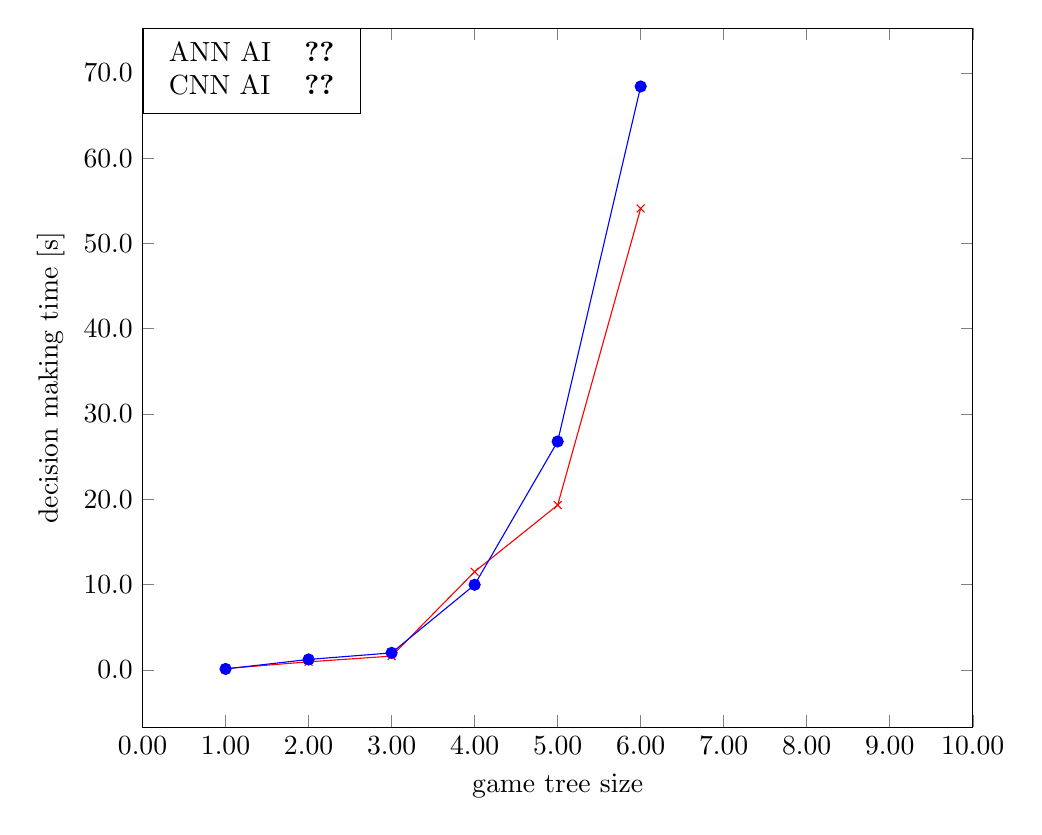
\begin{tikzpicture}
\begin{axis}[
    name=move-making-time-consumption,
    xmin=0, xmax=10,
    width=\textwidth,
    y tick label style={
        /pgf/number format/.cd,
            fixed,   % po zakomentowaniu os rzednych jest indeksowana wykladniczo
            fixed zerofill, % 1.0 zamiast 1
            precision=1,
        /tikz/.cd
    },
    x tick label style={
        /pgf/number format/.cd,
            fixed,
            fixed zerofill,
            precision=2,
        /tikz/.cd
    },
    xlabel={game tree size},
    ylabel={decision making time \lbrack s\rbrack}
]
\addplot [red, mark=x, domain=1:6]table{1 0.169
                2 0.958 
                3 1.628 
                4 11.521 
                5 19.331
                6 54.098
};\label{ann-ai}
\addplot [blue, mark=*, domain=1:6]table{1 0.122
                2 1.235 
                3 2.004 
                4 9.987 
                5 26.786
                6 68.4
};\label{cnn-ai}
\end{axis} 
\node[anchor=north west, draw=black, fill=white](legend) at (move-making-time-consumption.north west) {
    \begin{tabular}{ll}
        ANN AI & \ref{ann-ai}\\
        CNN AI & \ref{cnn-ai}\\
    \end{tabular}
};
\end{tikzpicture}
\caption{Time consumption in regards to game tree size.}
\label{fig:move-making-time-consumption}
\end{figure}
As it can be seen, both AI instances needs similar time to make decision. Slightly increase can be seen in case of instance using convolutional neural network but beginning three values are very similar. Testing has been performed up to game tree size of $6$. It has been performed this way because used local machine had not enough RAM memory to generate bigger game tree structure. By analyzing given plot, it is possible to choose the most optimal game tree size. The goal is to pick the biggest size possible witch acceptable decision making time. Because first big ,,spike'' in time variable can be seen in game tree size of $4$, it will be the best option to choose game tree size of $3$. Quick remark, results shown on \hyperref[fig:move-making-time-consumption]{fig. \ref*{fig:move-making-time-consumption}} explain perfectly, why the most often used game tree size is $3$ \cite{bib:article-chessai-in-game-analysis,bib:internet-step-by-step-chess-ai}. All of the following experiments will be performed with static game tree size of value $3$.

As it was mentioned in section \ref{sec:methodology}, this test set relies on playing against created AI instances in ,,player vs AI'' mode. As an first experiment, untrained AI instances has been tested. Unfortunately, results were terrible. Both AI instances performed randomly and all moves that it performed were suboptimal. This behavior is absolutely correct because like it was mentioned in section \ref{sec:learning-process-for-nn-instance}, all values for weights and biases are initialized with random values. Because parameters values are random, the same property is applied to neural network decisions. All games played in this scenario has been won by the human player. Additionally, only two times it was possible to win using \textbf{scholar's mate}. This is special type of checkmate, which has been achieved with only $4$ moves. Scholar's mate has been presented on \hyperref[fig:scholars-mate]{fig. \ref*{fig:scholars-mate}}. Achieving this situation was hard because it require enemy to perform one specific move, at the beginning of the game, which was almost impossible with randomly playing AI.
\begin{figure}
    \centering
    \newchessgame
    \hidemoves{1. e4 e5, 2. Qh5 Nc6, 3. Bc4 Nf6, 4. Qxf7}
    \showboard
    \caption{Scholar's mate example.}
    \label{fig:scholars-mate}
\end{figure}

Experiment performed on trained AI instances provided much more interesting results. Before moving to results description, it is important to mention who performed role of the player in this experiment. All manual games has been played by author of this thesis. ELO ranking score of this player is unknown but it is player who have over $10$ years of experience with chess. Considering this existence and gathered knowledge, tis player can be ranked as intermediate player. This is very good scenario for testing created AI instances. First parameter that will be used for specify play effectivity is \textbf{win ration}. Its value shows how many games has been won by AI. Win ration for both AI instances looks as follows:
\begin{itemize}
    \item Win ratio for AI using ANN: $\sim 45\%$,
    \item Win ratio for AI using CNN: $\sim 55\%$.
\end{itemize}
Achieved win ratio, for both neural networks looks very promising. It is even more promising when putting into consideration fact that this scores has been achieved while playing with intermediate chess player. Interesting property that has been observed during games is the fact that AI, containing artificial neural network, starts to make optimal moves in around $4th$ turn. Such behavior may indicate that this AI instance needs to be train more with increase number of ,,opening'' situation. This behavior can also be a good thing because it can put potential opponent in situation of feeling secure, which can result in making mistakes. In case of AI using convolutional neural network, also interesting behavior has been discovered. Player noticed that this AI instance was often aiming for performing scholar's mate. As it was mentioned in section \ref{sec:cnn-architecture}, first convolutional layer should aim in recognizing good opening patterns. Mentioned behavior can indicate that this goal has been achieved.

\subsection{Automated testing of AI instances}
This test set has also been divided into two sections. Both of the experiments was based on testing created AI instances in ,,AI vs AI'' mode. Unfortunately, first experiment that involved testing untrained AI instances, again didn't provided good results. All of played games has been interrupted after $50$ turns due to lack of the progression. Both AI instances has been playing randomly as it was described in section \ref{sec:manual-testing-ai}.

Second experiment provided much more promising results. Before presenting gathered results it is important to specify rules of the performed experiment. Because ,,AI vs AI'' mode provide user with limited control options (interrupt or continue game), following rules has been included:
\begin{itemize}
    \item interrupt game if $5$ sequential moves to not result in any progression,
    \item interrupt game at the end of $50th$ turn,
    \item interruption of the game will result in assuming that game result is draw.
\end{itemize}
Taking into consideration mentioned rules, $30$ games has been performed. Results of those games are presented in \hyperref[tab:ai-vs-ai-results]{tab. \ref*{tab:ai-vs-ai-results}} (result meaning: ,,1-0'' - AI using ANN wins, ,,0-1'' - AI using CNN wins, ,,1-2/1-2'' - draw).
\begin{table}
	\centering
	\caption{Results of AI vs AI games.}
	\label{tab:ai-vs-ai-results}
	\begin{tabular}{lll}
	\toprule
        \textbf{game id} & \textbf{result} & \textbf{description}\\
		\hline
			1 & 0-1 & None\\
        \hline
			2 & 0-1 & None\\
        \hline
			3 & 1-0 & None\\
        \hline
			4 & 1-2/1-2 & interrupted because of turn number limit\\
        \hline
			5 & 0-1 & None\\
        \hline
			6 & 1-0 & None\\
        \hline
			7 & 1-2/1-2 & interrupted because of turn number limit\\
        \hline
			8 & 0-1 & None\\
        \hline
			9 & 1-0 & None\\
        \hline
			10 & 1-0 & None\\
        \hline
			11 & 1-2/1-2 & interrupted because lack of progression\\
        \hline
			12 & 0-1 & None\\
        \hline
			13 & 0-1 & None\\
        \hline
			14 & 0-1 & None\\
        \hline
			15 & 1-0 & None\\
        \hline
			16 & 1-2/1-2 & interrupted because lack of progression\\
        \hline
			17 & 1-2/1-2 & interrupted because lack of progression\\
        \hline
			18 & 1-0 & None\\
        \hline
			19 & 1-0 & None\\
        \hline
			20 & 0-1 & None\\
        \hline
			21 & 1-0 & None\\
        \hline
			22 & 1-2/1-2 & interrupted because of turn number limit\\
        \hline
			23 & 0-1 & None\\
        \hline
			24 & 1-0 & None\\
        \hline
			25 & 0-1 & None\\
        \hline
			26 & 0-1 & None\\
        \hline
			27 & 0-1 & None\\
        \hline
			28 & 1-2/1-2 & interrupted because lack of progression\\
        \hline
			29 & 1-0 & None\\
        \hline
			30 & 0-1 & None\\
	\end{tabular}
\end{table}
By analyzing gather results it is possible to calculate win ratio of both AI instances. Draws were treated as both instances wins. Calculated win ratio looks as follows:
\begin{itemize}
    \item Win ratio for AI using ANN: $\sim 57\%$.
    \item Win ratio for AI using CNN: $\sim 67\%$.
\end{itemize}
Win ratios for both AI instances looks very promising and as it can be seen, both instances are on similar level. By analyzing played games, it was noticed that AI, that uses convolutional neural network, plays much better at the beginning of the game which in most cases resulted in wining whole game. In the section \ref{sec:manual-testing-ai}, it was mentioned that random plays at the beginning of the game, which artificial neural network performed, can be a good thing. Unfortunately, performed experiments shown that this tactic can work only against human opponent. This strategy can work better the lower the player experience level.



%\chapter{Experiments}
%
%This chapter presents the experiments. It is a crucial part of the thesis and has to dominate in the thesis. 
%The experiments and their analysis should be done in the way commonly accepted in the scientific community (eg. benchmark datasets, cross validation of elaborated results, reproducibility and replicability of tests etc).
%
%
%\section{Methodology}
%
%\begin{itemize}
%\item description of methodology of experiments
%\item description of experimental framework (description of user interface of research applications – move to an appendix)
%\end{itemize}
%
%
%\section{Data sets}
%
%\begin{itemize}
%\item description of data sets
%\end{itemize}
%
%
%\section{Results}
%
%\begin{itemize}
%\item presentation of results, analysis and wide discussion of elaborated results, conclusions
%\end{itemize}
%
%
%
%\begin{table}
%\centering
%\caption{A caption of a table is ABOVE it.}
%\label{id:tab:wyniki}
%\begin{tabular}{rrrrrrrr}
%\toprule
%	         &                                     \multicolumn{7}{c}{method}                                      \\
%	         \cmidrule{2-8}
%	         &         &         &        \multicolumn{3}{c}{alg. 3}        & \multicolumn{2}{c}{alg. 4, $\gamma = 2$} \\
%	         \cmidrule(r){4-6}\cmidrule(r){7-8}
%	$\zeta$ &     alg. 1 &   alg. 2 & $\alpha= 1.5$ & $\alpha= 2$ & $\alpha= 3$ &   $\beta = 0.1$  &   $\beta = -0.1$ \\
%\midrule
%	       0 &  8.3250 & 1.45305 &       7.5791 &    14.8517 &    20.0028 & 1.16396 &                       1.1365 \\
%	       5 &  0.6111 & 2.27126 &       6.9952 &    13.8560 &    18.6064 & 1.18659 &                       1.1630 \\
%	      10 & 11.6126 & 2.69218 &       6.2520 &    12.5202 &    16.8278 & 1.23180 &                       1.2045 \\
%	      15 &  0.5665 & 2.95046 &       5.7753 &    11.4588 &    15.4837 & 1.25131 &                       1.2614 \\
%	      20 & 15.8728 & 3.07225 &       5.3071 &    10.3935 &    13.8738 & 1.25307 &                       1.2217 \\
%	      25 &  0.9791 & 3.19034 &       5.4575 &     9.9533 &    13.0721 & 1.27104 &                       1.2640 \\
%	      30 &  2.0228 & 3.27474 &       5.7461 &     9.7164 &    12.2637 & 1.33404 &                       1.3209 \\
%	      35 & 13.4210 & 3.36086 &       6.6735 &    10.0442 &    12.0270 & 1.35385 &                       1.3059 \\
%	      40 & 13.2226 & 3.36420 &       7.7248 &    10.4495 &    12.0379 & 1.34919 &                       1.2768 \\
%	      45 & 12.8445 & 3.47436 &       8.5539 &    10.8552 &    12.2773 & 1.42303 &                       1.4362 \\
%	      50 & 12.9245 & 3.58228 &       9.2702 &    11.2183 &    12.3990 & 1.40922 &                       1.3724 \\
%\bottomrule
%\end{tabular}
%\end{table}  
%
%\begin{figure}
%\centering
%\begin{tikzpicture}
%\begin{axis}[
%    y tick label style={
%        /pgf/number format/.cd,
%            fixed,   % po zakomentowaniu os rzednych jest indeksowana wykladniczo
%            fixed zerofill, % 1.0 zamiast 1
%            precision=1,
%        /tikz/.cd
%    },
%    x tick label style={
%        /pgf/number format/.cd,
%            fixed,
%            fixed zerofill,
%            precision=2,
%        /tikz/.cd
%    }
%]
%\addplot [domain=0.0:0.1] {rnd};
%\end{axis} 
%\end{tikzpicture}
%\caption{Figure caption is BELOW the figure.}
%\label{fig:2}
%\end{figure}
%
